

\section{ER models (repetition \& continuation)}

%------------------------------------------------------------------------------
\begin{frame}{Repetition: ER terminology~\parencite[9--12]{chen1976}}
    % ----------------------------------------------
  \begin{columns}[T,onlytextwidth]
  \metroset{block=fill}
    \column{0.55\textwidth}\footnotesize
      \begin{block}{Entity (Entität)}
       An entity is a „thing“ which can be distinctly identified. A specific person, company, or event is an example of en entity.
      \end{block}

      \begin{alertblock}{Relationship (Beziehung)}
        A relationship is an association among entites. For instance, „father-son“ is a relationship between two „person“ enitities.
      \end{alertblock}

      \begin{exampleblock}{Entity Set (Entitätsmenge)}
        All entities of the same entity set have the same properties.
        %Alle Entitäten derselben Entitätsmenge haben dieselben Eigenschaften (properties). 
        
        „Entities are classified into different entity sets such as EMPLOYEE, PROJECT, and DEPARTMENT.“
      \end{exampleblock}

    % ----------------------------------------------

    \column{0.4\textwidth}

      \metroset{block=fill}

      \begin{block}{ER model elements}
      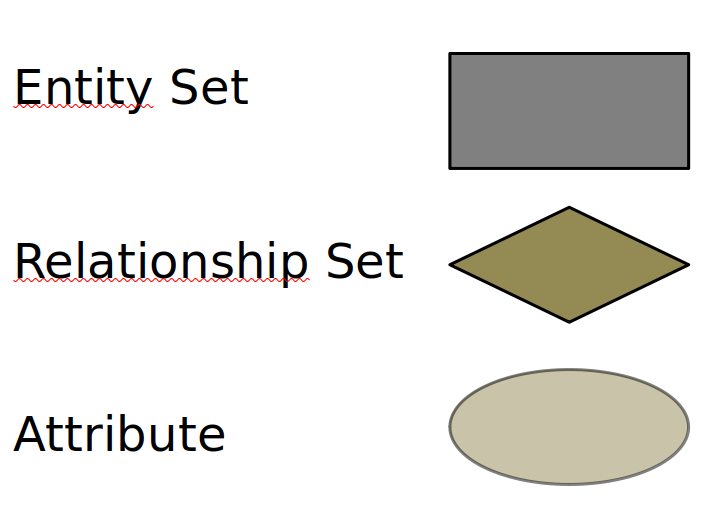
\includegraphics[width=0.9\textwidth]{img/er-modell.png}
      \end{block}
      
      \begin{block}{ER elements}
      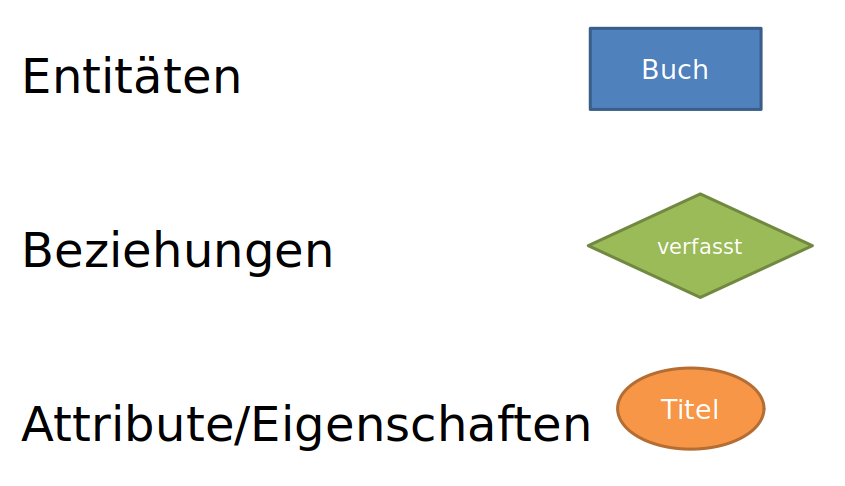
\includegraphics[width=0.9\textwidth]{img/er-bsp2.png}
      \end{block}
  \end{columns}

\end{frame}

%------------------------------------------------------------------------------
\begin{frame}{Repetition ER}
    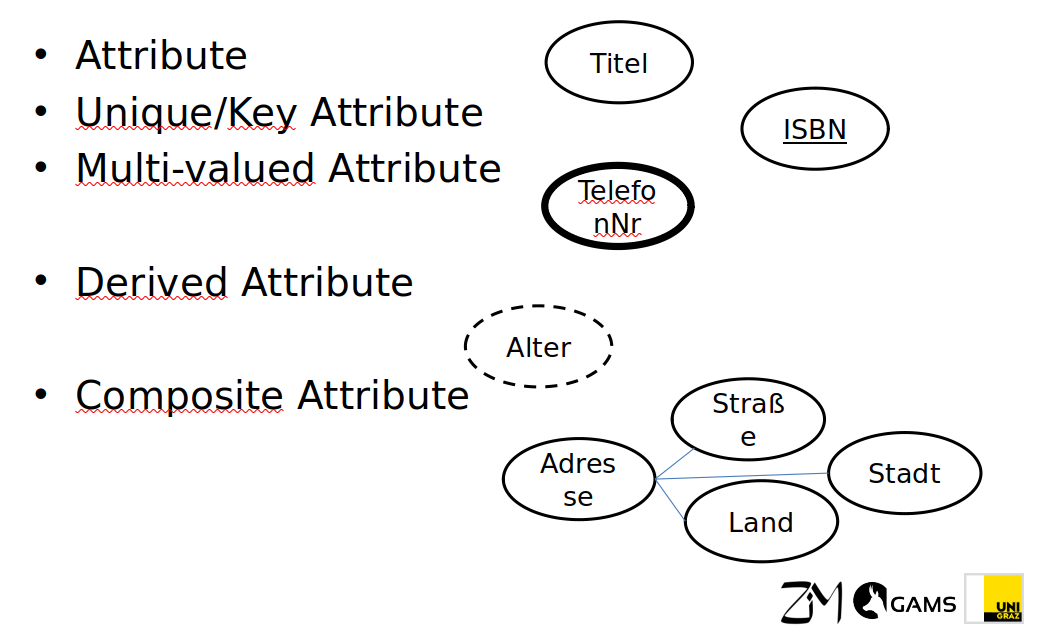
\includegraphics[width=\textwidth]{img/wdh-er-bestandteile.png}
\end{frame}


%------------------------------------------------------------------------------
\begin{frame}{Attribute values pairs and Primary Keys}
    Properties (Eigenschaften) are expressed by a attribute-value combination like so: 
    \begin{enumerate}
        \item The pen is blue = The `pen' entity has the attribute `color' with the value `blue'. 
        \item The pen is red = The `pen' entity has the attribute `color' with the value `red'. 
    \end{enumerate}

\metroset{block=fill}
\begin{exampleblock}{Primary Key: Identifying properties}
Entities and relationships can be uniquely identified via the value of one or multiple attributes combined. This attribute / the attribute combination is then called `primary key'. 
\end{exampleblock}
\end{frame}
%------------------------------------------------------------------------------
%\begin{frame}{Beispiel ER-Modell für ein Buch}    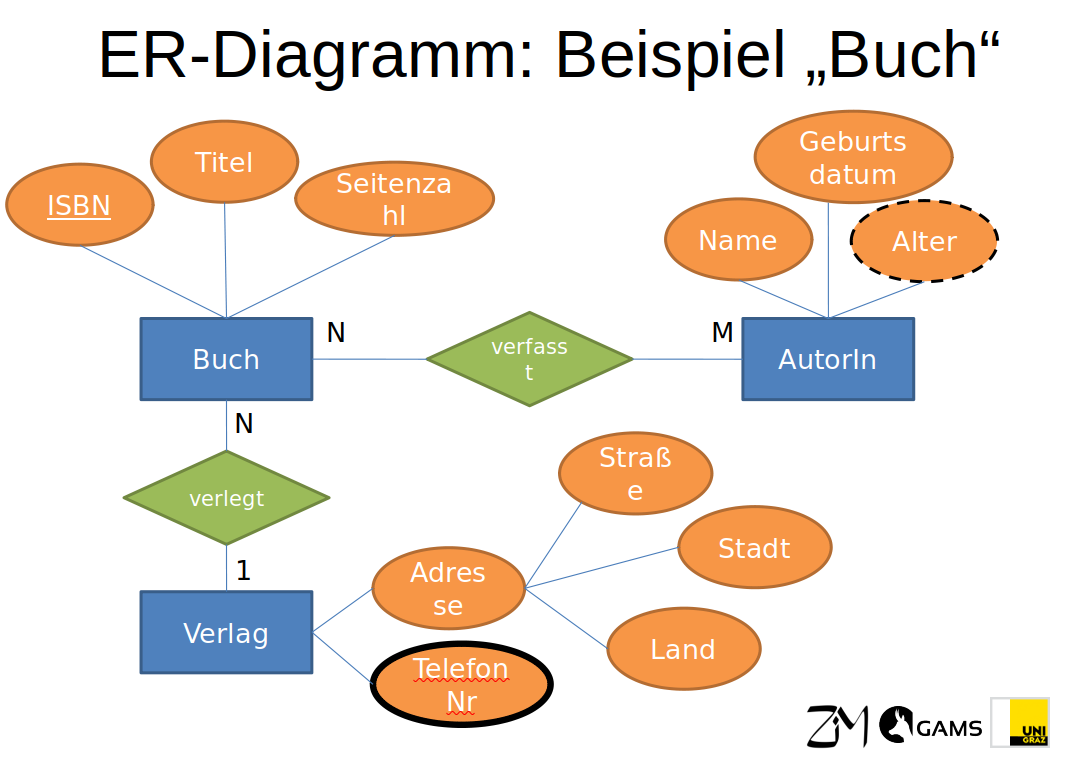
\includegraphics[width=\textwidth]{img/er-bsp3.png}\end{frame}


%------------------------------------------------------------------------------
\begin{frame}{Repetition exercise}
    % ----------------------------------------------
  \begin{columns}%[T,onlytextwidth]
  \metroset{block=fill}
    \column{0.45\textwidth}\footnotesize
    \begin{block}{A session of a university course}
    Such a session is defined by having:
    \begin{enumerate}
        \item students
        \item teachers
        \item seats
        \item a room
        \item in a building
    \end{enumerate}
    \end{block}

    % ----------------------------------------------

    \column{0.55\textwidth}
      \metroset{block=fill}\footnotesize
      \begin{exampleblock}{Exercise 1}
      \begin{enumerate}
          \item Which attribute can be used to describe these entities? %Mit welchen Attributen lassen sich diese Entitäten beschreiben?
          \item Using which attributes can the entities be uniquely identified? %Anhand welcher Attribute lassen sich die Entitäten jeweils identifizieren?
          \item Which relationships do they have amongst each other? %Welche Beziehungen existieren zwischen den Entitäten?
      \end{enumerate}
      $\to$ related to a normal in-person class % bezogen auf normalen Präsenzunterricht
      \end{exampleblock}
      \begin{exampleblock}{Exercise 2}
      How do we have to change this to accomodate distance learning or even a hybrid setting? % Wie müsste man das jetzt umändern, um auch Distance Learning einzukalkulieren?
      \end{exampleblock}
      \footnotesize
      $\to$ do this exercise in groups/pairs and create a visualisation of the results, for example using \href{https://erdplus.com/standalone}{the erdplus.com tool} (be ready to present this briefly) % Übung in Gruppen. Erstellen Sie, wenn möglich, eine Zeichnung / einen Screenshot der Resultate, der dann vorgestellt wird.
  \end{columns}

\end{frame}


%------------------------------------------------------------------------------
\begin{frame}{Solution: class session in ER (in-person) }
    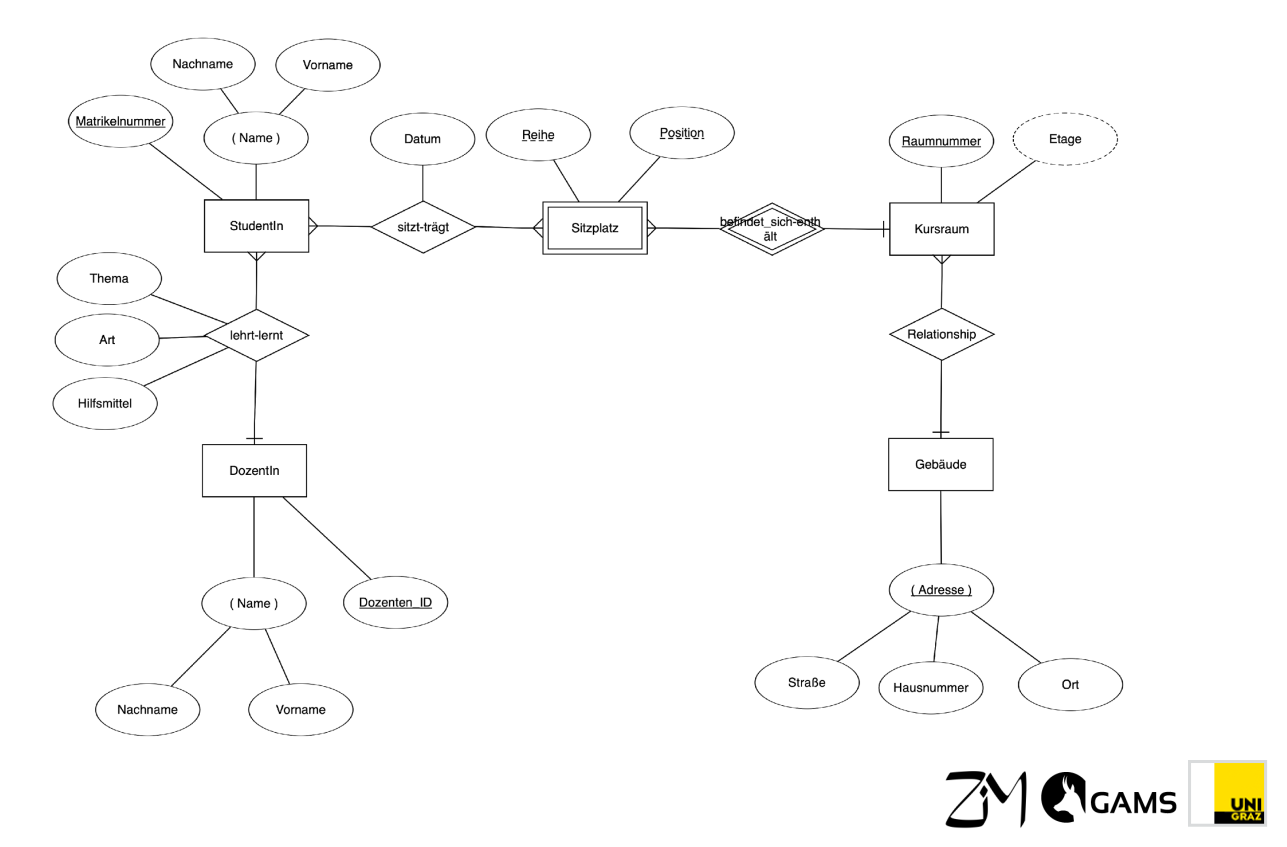
\includegraphics[width=\textwidth]{img/wdh-er-kursmodellierung.png}
\end{frame}


\subsection{ERM -- Tables \& relations}
%------------------------------------------------------------------------------

%------------------------------------------------------------------------------
\begin{frame}{From ER model to table format?}
    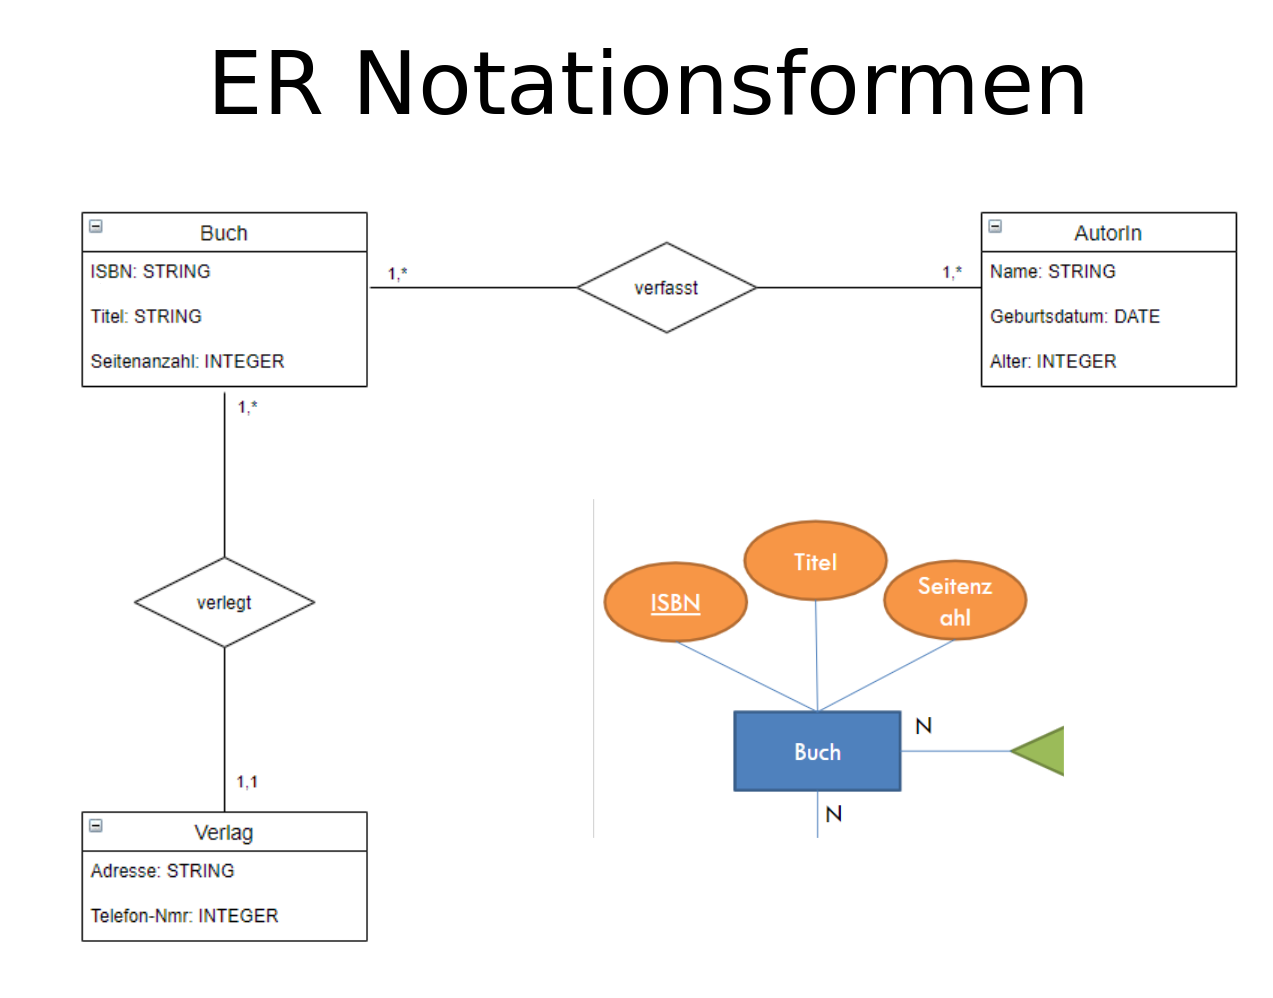
\includegraphics[width=\textwidth]{img/er-notation-buch.png}
\end{frame}

%------------------------------------------------------------------------------
\begin{frame}{Representation of ER models as tables}
    % ----------------------------------------------
  \begin{columns}[T,onlytextwidth]
  \metroset{block=fill}
    \column{0.4\textwidth}\footnotesize
    \begin{block}{Representation as tables}
    Entities and their relationships can be represented as tables. \\
    But where to put the attributes? 
    
    \end{block}

    % ----------------------------------------------

    \column{0.55\textwidth}
      \metroset{block=fill}
      \begin{exampleblock}{Handeling cardinalities}
      \begin{enumerate}\small
          \item Same book, multiple authors? (Why not just as an attribute?) 
          \item Same book, multiple genres? (entity or attribute?) 
          \item How to model the content of the book? (if at all?)
      \end{enumerate} \small
      $\to$ keep these questions in mind for a discussion later (on cardinality)
      \end{exampleblock}

  \end{columns}
\end{frame}

%------------------------------------------------------------------------------
\begin{frame}{Transform entities \& attributes to tables: e.g. class}
    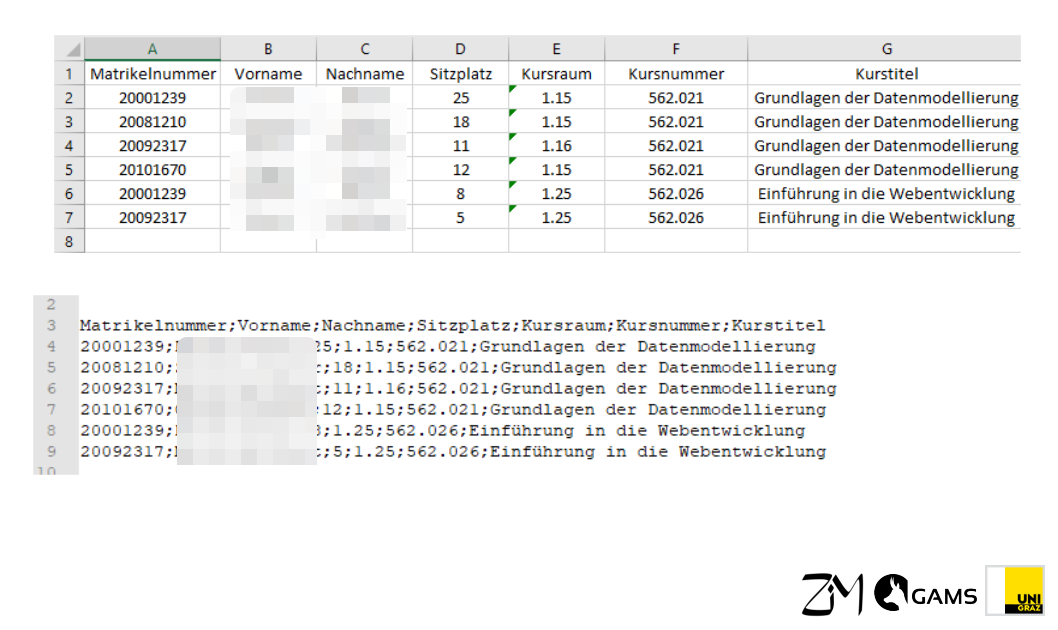
\includegraphics[width=\textwidth]{img/wdh-studierende-csv.png}
\end{frame}


%------------------------------------------------------------------------------
%\begin{frame}[standout]
    %\alert{Lektüre}-Zusammenfassung: \\
    %Chen, ER-Modelle \\[1em]
    %{\footnotesize Bitte \alert{\href{https://docs.google.com/presentation/d/1v_j9Jms21hZokX9hLJ_7kcnV63FJPHTHNowfLVLiYys/edit?usp=sharing}{hier im Google Slides zusammenfassen}}; 1 Person stellt dann vor. \\
    %Themen 1 und 2 für jene ohne größere DB-Vorwissen; 3 und 4 bitte möglichst, falls schon gewisses Programmierungs-/DB-Wissen vorhanden ist. \\
    %Aufgabe ist nicht, Details herauszupicken -- stark Technisches kann man auch weglassen. \alert{Bitte um Fokus auf die Verständnis-Aspekte.} Man kann gern zur Hilfe andere Materialien dazunehmen. Versuchen, den Mitstudierenden den Text möglichst verständlich aufzubereiten/zusammenzufassen. \\
    %Zeit ca. 20min}
%\end{frame}

%------------------------------------------------------------------------------
\begin{frame}{From real-world object to relational database?}
    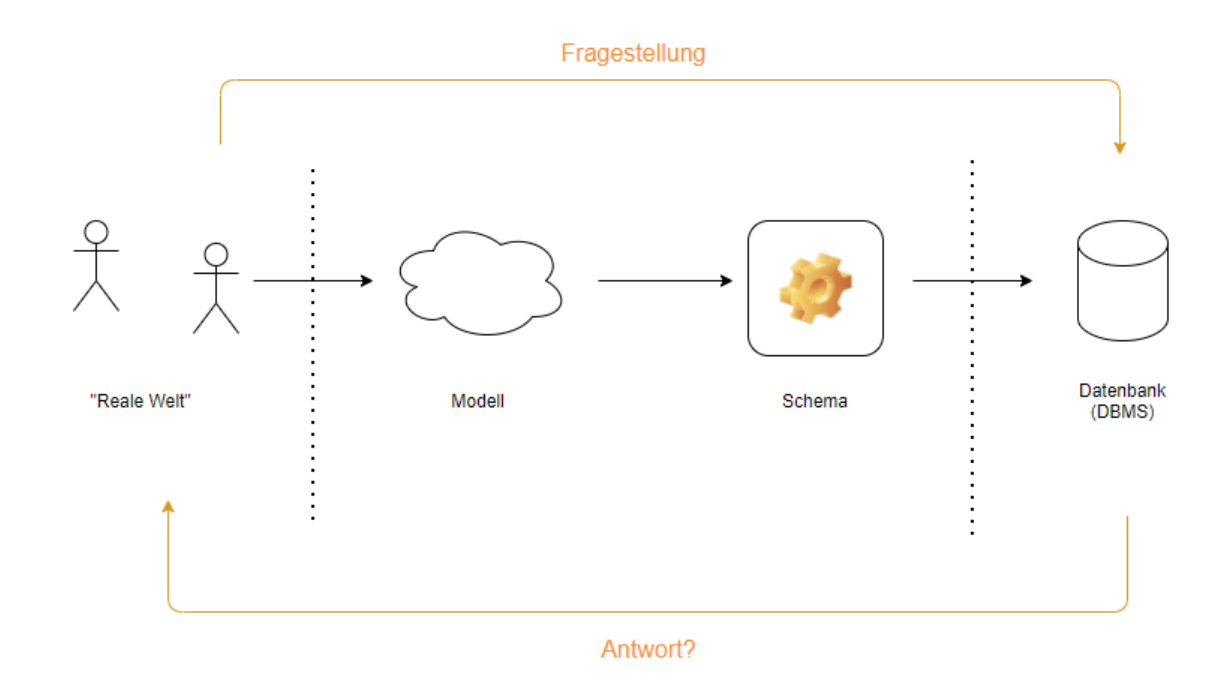
\includegraphics[width=\textwidth]{img/von-welt-zu-db.png}
\end{frame}

%------------------------------------------------------------------------------
\begin{frame}{Moving towards databases\dots}
    % ----------------------------------------------
  \begin{columns}[T,onlytextwidth]
  \metroset{block=fill}
    \column{0.4\textwidth}\footnotesize
    \begin{block}{Data analysis example: table of places}
    \begin{itemize}
        \item Are coordinates unique in the table or do some appear more than once? 
        \item Group and count places using the last digits of the latitude values, etc. 
        \item What visualizations would work for this data?
    \end{itemize}
    \end{block}

    % ----------------------------------------------

    \column{0.55\textwidth}
      \metroset{block=fill}
      \begin{exampleblock}{Preview: Relational Databases}
      \begin{enumerate}\small
          \item  \textbf{information and data modelling} = the way into the database
          \item \textbf{data analysis and retrieval} = query/retrieve information from the DB to answer questions: query structured data 
      \end{enumerate} 
      \end{exampleblock}
  \end{columns}
\end{frame}


%------------------------------------------------------------------------------
\begin{frame}[standout]
    \alert{Homework:} Install \alert{\href{https://sqlitebrowser.org/dl/}{SQLite}} \\[1em]
    {\footnotesize
    \begin{enumerate}
        \item maybe work in groups with those sharing your operating system (Linux, Windows, Mac)
        \item if you already have it, you can leave early -- but then figure it out yourself
        \item we don't necessarily need SQLiteBrowser (sometimes causes trouble)
        \item $\to$ there are tutorials; you can ask me or the others
        \item \alert{Tutorials: \href{https://www.tutorialspoint.com/sqlite/sqlite_installation.htm}{Tutorialspoint} | \href{https://www.sqlitetutorial.net/download-install-sqlite/}{SQLiteTutorial} | \href{https://github.com/sqlitebrowser/sqlitebrowser}{SQLiteBrowser Github}}
    \end{enumerate}
    }
\end{frame}



%------------------------------------------------------------------------------
%\begin{frame}[standout]
    %\alert{Reading:} \\ \small Bitte formieren Sie sich in Grupppen. Jede Gruppe erarbeitet eine Zusammenfassung eines Unterpunkts der Lektüre \alert{\href{https://docs.google.com/presentation/d/12w3XqjDO0IsLFwT0aFYiWED08WupCPxaswAEaxhqmuY/edit?usp=sharing}{in diesem GoogleDoc}} (Kapitel \emph{Grundlagen der Datenmodellierung}). \\ Jede Gruppe hat dafür max. 1 Slide zur Verfügung. Eine Person aus der Gruppe stellt diese am Ende dem Plenum vor. 
%\end{frame}


%------------------------------------------------------------------------------
%\begin{frame}[standout]
    %\alert{Reading} for next week: \\
    %DH-Einführung, Kapitel \emph{Datenmodellierung}
%\end{frame}

%------------------------------------------------------------------------------


%------------------------------------------------------------------------------
\begin{frame}{(materials for the) homework assignment}
\metroset{block=fill}
\begin{exampleblock}{Resources}
    \begin{itemize}\footnotesize
        \item \href{https://erdplus.com/standalone}{Tool for creating ER models}
        \item \href{https://www.geeksforgeeks.org/introduction-of-er-model/}{GeeksforGeeks tutorial/Intro to ER Models}
        \item \href{https://geobrowser.de.dariah.eu/}{DARIAH Geobrowser}
        \item \href{https://www.cloudbakers.com/blog/everything-you-didnt-want-to-have-to-know-about-csv}{Everything you didn't want to know about CSV}
    \end{itemize}
\end{exampleblock}

\begin{alertblock}{ER model homework assignment}
    \begin{enumerate}\footnotesize
        \item Create and visualize the model for your original (attribute class) using an ER diagram (like ERDplus) %Konzipieren und visualisieren Sie das Model Ihres Originals (Attributklasse) mithilfe des Entity-Relationship-Diagramms. (z.B. ERDplus siehe oben)
        \item Export it as an image and upload it on Moodle %Exportieren Sie ihr Diagramm als Bild und laden es auf Moodle hoch.
        \item In case of problems, help each other via Slack or in-person. %Bei Problemen können Sie sich auch gegenseitig im Hilfe-Forum unterstützen.
        \item \textbf{Bonus:} Look into the subject of cardinality and work it into your model. %Schauen Sie sich das Thema `Kardinalität' an bzw. erarbeiten es sich aus den Unterlagen und bauen Sie es in Ihr Modell ein. 
    \end{enumerate}
\end{alertblock}
\end{frame}

%------------------------------------------------------------------------------
%\begin{frame}[standout]
    %\alert{Lektüre} auf nächste Einheit: \\
    %Chen, ER-Modelle 
%\end{frame}


%------------------------------------------------------------------------------
\section{Cardinality}
\begin{frame}[allowframebreaks]{Cardinalities}
\metroset{block=fill}
    "cardinality" =  the number of entities participating in a relationship where  \textit{n} \& \textit{m} stand for an arbitrary number.

\begin{block}{Types of relationships}
 \textbf{1:1} $\to$ exactly one entity participates in the relationship. %Es gibt genau je eine Entität, die an der Beziehung beteiligt ist.
 
 \textbf{1:n} $\to$ There can be an arbitrary number of entities (on the n-side) for each single entity on the 1-side. %Für jede Entität auf der 1-Seite der Beziehung kann es beliebig viele Entitäten auf der n-Seite geben.
 
 \textbf{n:m} $\to$ There can be an arbitrary number for each entity on the n-side on the m-side and vice versa. %Für jede Entität auf der n-Seite der Beziehung kann es beliebig viel Entitäten auf der m-Seite geben und umgekehrt.
\end{block}

\begin{center}
  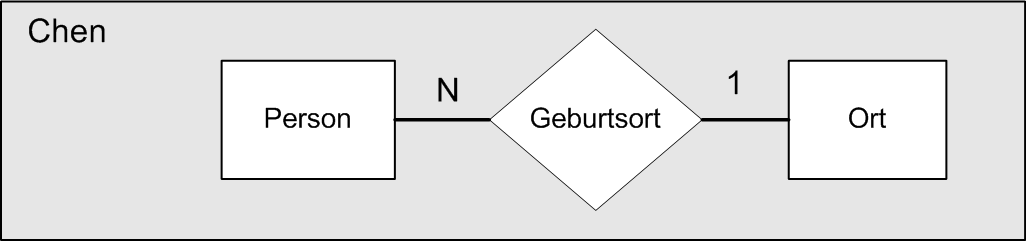
\includegraphics[width=0.7\textwidth]{img/ERD_Darstellungen_Chen.png}
\end{center}

\framebreak
\begin{block}{Minimal cardinalities} 
\textbf{0} $\to$ there doesn't have to be an entity on this side of the relationship. (=\textit{optional})

\textbf{1} $\to$ There has to be at least one entity on this side of the relationship.  (=\textit{obligatory})
\end{block}

\begin{center}
    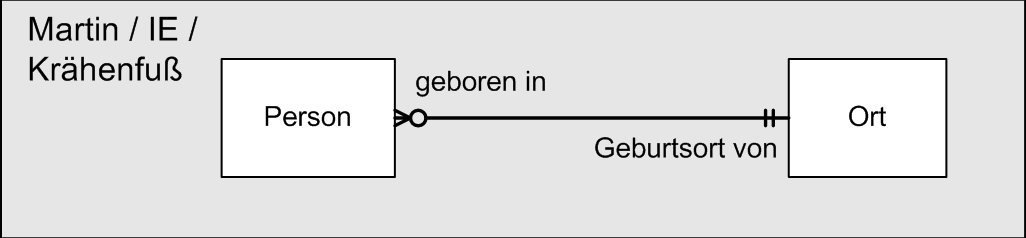
\includegraphics[width=0.7\textwidth]{img/ERD_Darstellungen_Crowfoot.png}
    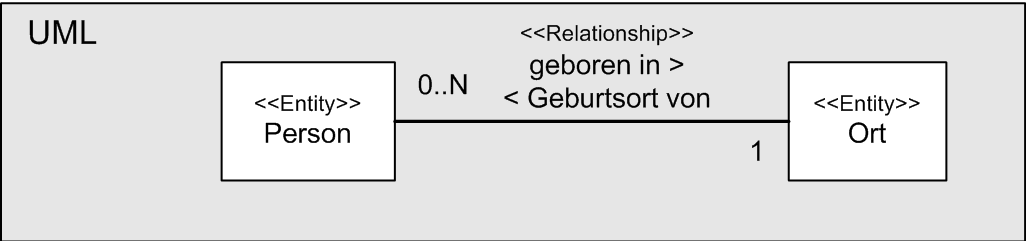
\includegraphics[width=0.7\textwidth]{img/ERD_Darstellungen_UML.png}
\end{center}

\end{frame}



%------------------------------------------------------------------------------
\begin{frame}{ER advanced}
    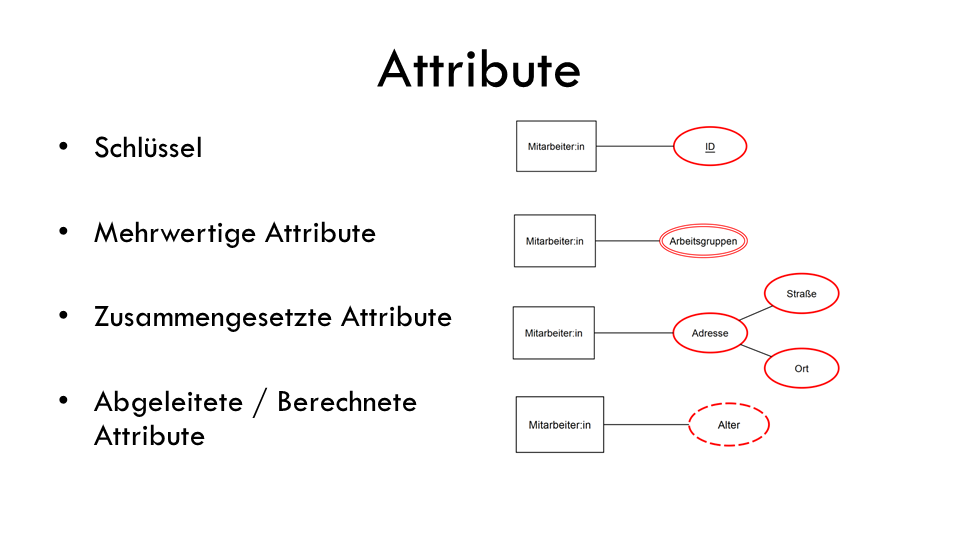
\includegraphics[width=\textwidth]{img/attribute.png}
\end{frame}


%-------------------------------------------------
\begin{frame}[allowframebreaks]{ER advanced}
    \begin{itemize}
        \item \textbf{identifying attributes (``keys``)}: these values are unique within the entity class and can thus be used to identify single entities. 
        \item \textbf{multivalued attributes}: attributes containing more than one atomic value.
        \item \textbf{derived attributes}: attributes which can be calculated from other attributes.
        \item \textbf{composite attributes}: attributes consisting of multiple parts.
    \end{itemize}
    
    \framebreak
    
    \begin{itemize}
        %\item \textbf{Attribute von Beziehungen}: Auch Beziehungen können Attribute haben.
        \item \textbf{n-ary relationships}: a relationship set can connect multiple entity sets (in principle). 
        \item \textbf{weak entity}: can only exist if there is a relation to another entity (room in building) but the key depends on the key of another relationship (Chen notation: double border). They have no properties of their own by which they can be identified (have no primary key). They are defined only by their relationship to a strong entity. Example: relatives of an employee in a company.
    \end{itemize}
\end{frame}
%\end{comment}

%-------------------------------------------------
    
\begin{frame}{n-ary relationships}
\begin{center}
    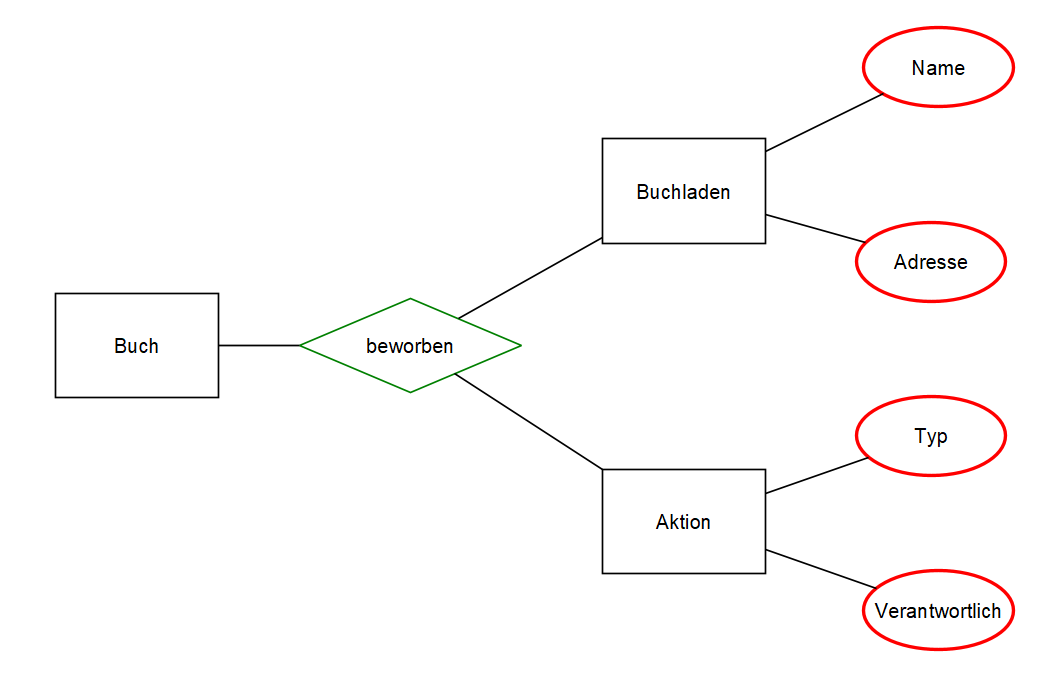
\includegraphics[width=0.9\textwidth]{img/n-ary-relationship.png}
\end{center}    
\end{frame}

%------------------------------------------------------------------------------
\begin{frame}{How to represent entities going from ER to table?}
    \begin{itemize}
        \item \textbf{entity} $\to$ table
        \item \textbf{attribute} $\to$ column
        \begin{itemize}
            \item multi-valued attributed $\to$ helper table
        \end{itemize}
        \item \textbf{relationship}
            \begin{itemize}\footnotesize
                \item \textbf{1:1} $\to$ Key of one entity (table) is stored as reference (`foreign key'/`Fremdschlüssel') in the other table as a column/attribute of its own 
                \item \textbf{1:n} $\to$ key of the 1-ary entity/table stored as reference in the n-ary table/entity 
                \item \textbf{n:m} $\to$ table of its own containing the keys of both related entities
                \item \textbf{n-ary relations} $\to$ helper table containing the keys of all entities as columns 
                \item \textbf{relationship attributes} $\to$ helper table with the keys of participating entities and columns for the attributes 
                \item \textbf{multi-valued attributes} $\to$ helper table with entity key as foreign key (like a 1:n relation) and a column for the attribute 
                \item \textbf{composite attributes} $\to$ helper table with entity key as foreign key (like a 1:n relation) and columns for the partial attributes 
            \end{itemize}
    \end{itemize}
\end{frame}

